% MediSense-Cardio -- IEEE conference paper, REBUILT 2026-11-14 from results/FINAL_NUMBERS.md (sections 1-10.10); UPDATED 2026-11-16 with 10.11-10.20 and 11 (printed paper, learned intervals, pattern findings, risk pilot 1). Risk pilot 2 added 2026-11-16 (failed, FINAL_NUMBERS 10.21).
% This file replaces main.tex (the September draft, 50 records, first sweep only). main.tex is kept unchanged for reference.
% Every number below is taken from results/FINAL_NUMBERS.md; numbers listed in its section 8 are never quoted.
% Not compiled locally (no LaTeX on this machine): upload docs/paper/ to Overleaf, set main_v2.tex as the main document, pdfLaTeX.
% Placeholders: title (working), author block, funding line -- deferred by the team.
% Thresholds named "pre-set rule" are the team's proposal and are NOT approved by the guide.

\documentclass[conference]{IEEEtran}
\IEEEoverridecommandlockouts
\usepackage{cite}
\usepackage{amsmath,amssymb,amsfonts}
\usepackage{graphicx}
\usepackage{textcomp}
\usepackage{xcolor}
\usepackage{booktabs}
\usepackage{url}

\begin{document}

\title{From Paper to Patient: Quantifying and Mitigating Digitization-Induced False Reassurance in Automated ECG Explanation\\
\large \textit{[Working title -- to be confirmed]}}

% TODO: author block, affiliations, emails, funding line.
\author{
\IEEEauthorblockN{Author Name(s) [TODO]}
\IEEEauthorblockA{\textit{School of Computer Science and Engineering [TODO]} \\
\textit{VIT-AP University [TODO]} \\
Amaravati, India \\
email@example.com [TODO]}
}

\maketitle

\begin{abstract}
Many electrocardiograms (ECGs) exist only as printouts or phone photographs, and programs that digitize them are used to measure heart rate and intervals. We ask how photo damage changes those measurements, how a user can be warned, and which measurements and findings can be shown safely. We use an open-source digitizer (Open-ECG-Digitizer) unchanged on PTB-XL recordings drawn as paper-style pages, on competition captures, on our own phone photographs of a screen, and on printed pages photographed by another person. Every rule was written before its result was seen, and negative results are reported as measured. In simulation, only very low resolution and heavy blur often made the heart rate wrong (47\% and 17\% of held-out pages). A score from the picture alone could not predict failures, but a traffic light computed from the digitized signal could: on competition captures GREEN readings were wrong in 0.2\% (2 of 917). Straightening the photographed page cut bad readings from 14 to 2 of 40 photos (exact paired $p=0.0005$); on printed paper it did so for 66 recompressed photos (31 to 15, $p=0.0004$) but not for 22 straight full-resolution photos (3 to 2), and 2 of 19 GREEN readings there were wrong. Against commercial reference values, heart rate, PR interval and frontal QRS axis met pre-set rules for straightened photos, while QT, QRS duration and P- and T-wave amplitude did not, because slope and bias checks exposed errors that a small average error hid. Networks trained only on public data found infarction and ST/T patterns on new photos (AUROC 0.81--0.84), while conduction held on screen photos but failed on printed paper, and two mortality-risk pilots failed their pre-set rules (one year, ECG only: AUROC 0.71 against 0.80 for age alone; five years, ECG plus age: 0.83 against 0.82, a gain of +0.013 that is not significant) and no risk is shown. The results hold for one digitizer and two phones; the tool is a research prototype, not a medical device.
\end{abstract}

\begin{IEEEkeywords}
electrocardiogram, ECG digitization, image damage, reliability check, false reassurance, validation
\end{IEEEkeywords}

\section{Introduction}

A printed or photographed ECG is often read outside a clinic: a photo sent over a messaging app, a printout from a home device, an image uploaded to a service that explains it in plain language. Such systems first turn the image back into signals. Open tools can now do this at scale \cite{ref5,ref3,ref53}, and public data and challenges have driven rapid progress \cite{ref1,ref2,ref4}, building on earlier image-processing work \cite{ref6,ref9}. These tools are usually validated on clean scans, although a published letter argues that image quality is crucial for AI-enabled digitization and interpretation of ECGs in occlusion myocardial infarction \cite{ref61}. What happens to the numbers read from a damaged photograph, and what a user should be told, is far less studied.

We study this with one fixed digitizer and three questions. \emph{(Q1)} Which kinds of photo damage make a measurement wrong? \emph{(Q2)} Can a reliability check warn the user, and from what? \emph{(Q3)} Which individual measurements can be shown at all? The third question matters because a measurement with a small average error can still hide large errors where they matter most, such as a long QT interval or a wide QRS complex, and a falsely reassuring number is worse than no number.

\textbf{Contributions.} (1) A measured account of which damage types break heart rate on a held-out set, and a negative result for a picture-only warning. (2) A traffic light computed from the digitized signal, frozen before real data were scored. (3) A page-straightening step confirmed on new photographs with a rule fixed beforehand. (4) A per-measurement validation with pre-set rules that accepts heart rate, PR interval and axis for straightened photos and rejects QT, QRS duration and P- and T-wave amplitude. (5) A demonstration that shows only validated information in fixed, tested wording. (6) Further tests with rules fixed beforehand: photographs of printed pages from another phone, a network for QRS duration and QT trained on public data only, ECG-pattern findings, and a mortality-risk pilot that failed and is reported as a negative result.

The closest published work studies the robustness of digitizers to image damage \cite{ref54} and adds a vision-language quality-assurance module \cite{ref55}. Our work differs in three ways: the digitizer is fixed and unmodified, each clinical measurement is evaluated separately against reference values under rules written down in advance, and the user-facing output is designed so that an unreliable result is never presented as reassuring.

\section{Related Work}

\textbf{ECG digitization.} The Moody PhysioNet Challenge 2024 asked teams to digitize and classify ECG images \cite{ref2}, supported by ECG-Image-Kit, which draws realistic pages from recordings with artifacts such as wrinkles and stains \cite{ref1}. Open-ECG-Digitizer \cite{ref5}, ECGtizer \cite{ref3} and the winning Challenge entry \cite{ref53} are recent open pipelines. A large paired image database of real captures followed \cite{ref4}.

\textbf{Quality assessment and abstention.} Much work scores the quality of ECG \emph{signals} \cite{ref12,ref13,ref14}. Selective prediction and deferral \cite{ref23,ref24} aim to let a system decline to answer; a clinician study found that abstention reduced the harm of automation bias overall but increased missed problems \cite{ref26}. We therefore make no claim that a warning helps patients.

\textbf{Plain-language explanations.} Patient-facing explanations by language models are an active area \cite{ref33}. We avoid free text: every sentence shown comes from a fixed, tested list.

\section{Method}

\subsection{Data and reference values}
Recordings come from PTB-XL \cite{ref45}, 21{,}799 ten-second 12-lead records; pages are drawn from the 100~Hz version. Reference interval and axis features come from PTB-XL+ \cite{ref46}, which provides measurements from two commercial algorithms (12SL and Glasgow). We fixed random subsets in advance: the first 50 recordings (development), 100 further recordings (held-out; 148 of 150 reliable), 140 recordings of the competition image dataset (9 capture types each, 1{,}260 images), own phone photographs of 30 and then 20 recordings (60 and 40 photos), and later sealed sets of 100 fresh recordings each. The reference heart rate is measured on the recording the page was drawn from by the same code. A recording is reference-uncertain when its 100~Hz and 500~Hz versions disagree by more than 5~bpm (20 of 150); conclusions are checked with and without them.

\subsection{Pages, damage and real captures}
Pages are drawn with a patched copy of ECG-Image-Kit \cite{ref1} at 25~mm/s, 10~mm/mV and 200~dpi (one pixel $=5.08$~ms $=0.0127$~mV), 2200$\times$1700 pixels. Six damage types are applied at five levels: Gaussian blur, rotation (2--16$^\circ$), JPEG compression, low resolution (shrunk to 75--15\%), a left-to-right brightness ramp, and a faded grid. Real captures are the competition photographs and scans (print-scan, phone photos of print and of a screen, stained, damaged, mouldy), and our own phone photographs of pages shown on a laptop screen, taken straight on and from about 30$^\circ$.

\subsection{Digitizer and measurements}
Open-ECG-Digitizer \cite{ref5} is used unchanged (commit 97a15087, published weights, one settings file). It returns 12 leads at 1{,}000~Hz in microvolts. Heart rate uses NeuroKit2\footnote{\url{https://github.com/neuropsychology/NeuroKit}} R-peaks on cleaned lead~II, for the reference and the digitized signal. A reading is \emph{wrong} if it differs by more than 5~bpm and has \emph{no usable heart rate} if fewer than 3 beats are found; \emph{bad} means either. PR, QT, QRS duration, P- and T-wave amplitude are measured from a median beat per lead with our own code (QRS onset by a slope fraction, T end by the tangent method, P onset by tangent); axis uses the net QRS deflection of the six limb leads by least squares. Statistics: Wilson 95\% intervals; resampling of whole recordings; exact McNemar test with Holm correction; Bland--Altman; AUC; cross-validation that holds out whole recordings.

\subsection{Reliability check and straightening}
Fifteen features computed only from the digitized signal (readable share, beat count, RR variation, amplitude, high-frequency share, Einthoven and Goldberger consistency, agreement of beat counts across leads) feed a logistic regression trained once on simulated damage and then frozen. AMBER begins at the 10th percentile of scores of wrong readings in training (0.2585), RED at the lowest score above which half the readings are wrong (0.7823); fewer than 3 beats is RED; a guard turns GREEN into AMBER when a feature is outside its training range. The straightening step finds the page (Otsu threshold, largest quadrilateral) and maps its corners to 2200$\times$1700 by a perspective transform.

\subsection{Validation of each measurement}
A measurement is shown only if it passes a rule written before the test, on a development set, a sealed test and a confirmation set, each run once. Calibration may only add an offset, never rescale, because rescaling shrinks values toward the mean and hides errors. Rules (the team's proposal, not guide-approved): median error and share within a tolerance, absolute bias, at least 90\% of cases with a value, a slope of the measured value on the 12SL value of at least 0.8, and tail checks for long QT, short QT and wide QRS (Table~\ref{tab:rules}). Measurements for which the two commercial algorithms disagree strongly (P and T duration, ST amplitude) were not attempted.

\subsection{Further tests and models}
Printed pages were photographed by one other person with an unknown phone and sent by a messaging app (80 photos of 20 printed pages, then 40 more); they are never pooled with our own photos. A photo taller than wide is first turned by 90$^\circ$ because the page finder expects a landscape photo. Three small one-dimensional networks were trained \emph{only} on public datasets (PTB-XL, and for the risk pilot CODE-15\%), never on our own pages or photos: one for QRS duration and QT (12SL labels, fixed digitizer emulation in training, an offset but no fitted slope), one for six ECG patterns (normal, infarction MI, ST/T change STTC, conduction CD, hypertrophy HYP, atrial fibrillation AF; folds 1--8 for training, fold 9 for calibration, fold 10 as benchmark, with our digitized pages T2 and straightened photos T3 as tests), and one for death within one year from the ECG alone (patient-level split, a test split touched once). Each model was trained once and tested once, and a finding is shown only if it meets pre-set rules (at least 20 positives, AUROC $\ge0.80$ with the interval's lower end above 0.70 on drawn pages; for photos also at least 20 positive photos and AUROC $\ge0.75$).

\begin{table}[t]
\caption{Pre-set pass rules (team proposal)}
\label{tab:rules}
\centering
\small
\begin{tabular}{lll}
\toprule
Measure & Typical error / within / bias & Extra \\
\midrule
QT & 20 / 40 / 10 ms & slope $\ge$0.8, tails \\
QRS & 10 / 20 / 5 ms & slope $\ge$0.8, tails \\
PR & 20 / 40 / 10 ms & steady rhythm \\
Axis & 10$^\circ$ / 30$^\circ$ (90\%) / 10$^\circ$ & categories $\ge$90\% \\
P amp. & 0.03 / 0.06 / 0.015 mV & slope $\ge$0.8 \\
T amp. & 0.05 / 0.10 / 0.03 mV & slope, sign $\ge$90\% \\
\bottomrule
\end{tabular}
\end{table}

\begin{figure}[t]
\centering
\includegraphics[width=0.95\columnwidth]{figures/fig_pipeline.png}
\caption{The method as a flow of steps.}
\label{fig:pipeline}
\end{figure}

\section{Results}

Each result is labelled PRE-SPECIFIED (rule written before the result), EXPLORATORY (idea came after earlier data) or POST HOC.

\subsection{Which damage makes heart rate wrong (pre-specified)}
On the held-out 100 recordings at the worst level, only very low resolution and heavy blur gave many wrong heart rates (Table~\ref{tab:damage}, Fig.~\ref{fig:damage}); the result held with and without reference-uncertain recordings. Rotation to 16$^\circ$ did not give wrong readings; it gave no output on 19 of 99 pages. A repeat run of 12 recordings changed the bad label on 0 of 156 images.

\begin{table}[t]
\caption{Wrong heart rate at the worst level, held-out 100}
\label{tab:damage}
\centering
\small
\begin{tabular}{lrl}
\toprule
Damage & Wrong & 95\% interval \\
\midrule
Clean page & 3/99 = 3.0\% & 1.0--8.5\% \\
Low resolution (15\%) & 47/99 = 47.5\% & 37.9--57.2\% \\
Blur (21$\times$21) & 17/99 = 17.2\% & 11.0--25.8\% \\
Rotation (16$^\circ$) & 0/99 (19 no output) & 0.0--3.7\% \\
JPEG (quality 3) & 0/99 & 0.0--3.7\% \\
Brightness ramp & 1/99 = 1.0\% & 0.2--5.5\% \\
Faded grid & 3/99 = 3.0\% & 1.0--8.5\% \\
\bottomrule
\end{tabular}
\end{table}

\begin{figure}[t]
\centering
\includegraphics[width=0.95\columnwidth]{figures/fig_wrong_by_damage.png}
\caption{Wrong heart rate at the worst damage level (95\% intervals).}
\label{fig:damage}
\end{figure}

\subsection{A picture-only warning fails; the digitized output works (pre-specified, then exploratory)}
A detector from five picture scores reached AUC 0.858 (0.81--0.91) on the held-out set, but an oracle told only the damage type and level reached 0.827. Inside one damage type and level it was at chance (0.521 for resolution level~5, 0.476 for blur level~5), it did not generalise to an unseen damage type, and it scored AUC 0.516 on real captures. The held-out set held 86 wrong readings, fewer than the 100 needed for a firm verdict, so the claim is inconclusive; the honest reading is negative. In contrast, 15 features of the digitized signal gave AUC 0.926 (0.89--0.95), and 0.873 and 0.892 inside resolution and blur level~5 (exploratory). The cost: right readings were flagged for 67\% (45/67) on atrial fibrillation or flutter recordings, because a truly irregular rhythm looks like a failed read.

\subsection{Real captures (exploratory, post hoc)}
No capture type of the competition data was significantly worse than the clean page in wrong heart rate; the one large effect was no output for phone photos of a screen (53/140 = 38\%, against 1\% clean). The clean page itself gave a wrong heart rate for 16/140 = 11\% of recordings: the digitizer drew the right waveform (median correlation 0.98) and the fault lay in a fragile one-number heart rate from raw beat finding. Cleaning the signal before beat finding, on both sides, cut wrong readings from 168 of 1{,}203 to 46 of 1{,}201 (post hoc; both versions are reported).

\subsection{Traffic light (exploratory)}
Frozen before any real data were scored, the light separated wrong readings (Table~\ref{tab:light}). On competition captures GREEN readings were wrong 0.2\% (2/917); on own photos GREEN 0/22 and RED 13/17. Intervals treat images as independent and are optimistic; fewer than 100 wrong readings make this descriptive.

\begin{table}[t]
\caption{Wrong heart rate by light (images with an output)}
\label{tab:light}
\centering
\small
\begin{tabular}{llrl}
\toprule
Data & Light & Readings & Wrong (95\%) \\
\midrule
Competition & GREEN & 917 & 2 (0.2\%, 0.1--0.8) \\
 & AMBER & 204 & 14 (6.9\%, 4.1--11.2) \\
 & RED & 82 & 30 (36.6\%, 27.0--47.4) \\
Own phone, set 1 & GREEN & 22 & 0 (0.0\%, 0--14.9) \\
 & AMBER & 15 & 1 (6.7\%) \\
 & RED & 17 & 13 (76.5\%, 52.7--90.4) \\
\bottomrule
\end{tabular}
\end{table}

\subsection{Straightening the photograph (confirmed)}
On 60 photos straightening cut bad readings from 20 to 2 (exploratory: the fix was designed on these photos). On 40 new photos of 20 new pages, with the rule fixed before the photos existed, bad readings fell from 14 to 2 of 40 (newly bad 0, newly good 12; exact McNemar $p=0.0005$): the fix is \emph{confirmed}. Angled shots fell from 10/20 to 1/20. Enlarging alone gave 13/40. No bad reading received GREEN. The two remaining bad readings belong to one page that the digitizer misreads whatever the photo. In an added simulation of 120 phone photographs of 60 sealed pages (a script, not a camera; rule fixed before the photographs existed, test run once), bad readings fell from 64 to 21 (newly bad 5, newly good 48; exact $p=7\times10^{-10}$), but 1 of 71 GREEN readings on the straightened photographs was wrong, so GREEN is not a guarantee.

\subsection{Per-measurement validation (exploratory)}
The standard wavelet method in NeuroKit2 failed even on original signals (typical error QT 36~ms, PR 78~ms, QRS 84~ms against 12SL). Our median-beat methods gave the results in Table~\ref{tab:valid}. \textbf{PR} met the rule on held-out original, held-out digitized and straightened phone photos (typical error 7.3~ms on digitized pages, 12.0~ms on photos), but only after straightening and only for rhythms in which 12SL finds a P wave: for atrial fibrillation or flutter our method still produced a number for all 6 held-out pages, so PR is hidden when the beat spacing varies (rr\_cv $>0.12$), a precaution calibrated on 14 cases. \textbf{Axis} met the rule on 100 fresh pages and 100 straightened photos (typical error 4.4$^\circ$, 95\% within 30$^\circ$); one recording was wrong by about 120$^\circ$ and detection of right axis deviation is not shown to work. \textbf{QT} met the error rule on fresh drawn pages (8.8~ms) but not on photos (14.9~ms, bias $-16.5$~ms), and its slope on 12SL was 0.68--0.69: a true QT of 350~ms or less was overestimated by 23--27~ms. A third attempt with a combined-lead method could not freeze a QT candidate (none reached slope 0.8). \textbf{QRS duration} failed in all three attempts: on 100 fresh pages the digitized-page test met the rule (5.5~ms) but the original-signal check had slope 0.79; on 40 straightened photos the bias was $+15.4$~ms and the slope 0.74. \textbf{P-wave amplitude} met the rule on 100 sealed pages (0.012~mV, slope 0.99) but on 40 straightened photos the slope was 0.77; \textbf{T-wave amplitude} reached a slope of only 0.68 in development and was not tested. ST segment, P duration and T duration were not attempted.

\begin{table}[t]
\caption{Validation against 12SL (typical error; slope on 12SL; rule)}
\label{tab:valid}
\centering
\small
\begin{tabular}{llll}
\toprule
Measure & Test set & Error; slope & Rule \\
\midrule
PR & digitized pages & 7.3 ms & met \\
PR & photos, straightened & 12.0 ms & met \\
PR & photos, not straight. & 8.7 ms; 67\% value & not met \\
Axis & fresh pages & 3.8$^\circ$ & met \\
Axis & photos, straightened & 4.4$^\circ$ & met \\
Axis & photos, not straight. & 4.9$^\circ$ & not met \\
QT & fresh pages & 8.8 ms; 0.69 & slope fails \\
QT & photos, straightened & 14.9 ms & not met \\
QRS & photos, straightened & 6.2 ms; 0.74 & not met \\
P amp. & sealed pages & 0.012 mV; 0.99 & met \\
P amp. & photos, straightened & 0.014 mV; 0.77 & not met \\
T amp. & development & slope 0.68 & stopped \\
\bottomrule
\end{tabular}
\end{table}

\subsection{Printed paper, another phone (exploratory)}
Photos of 20 printed pages taken by another person were matched to their pages by image content (checked against 16 of 16 page identifiers read by eye); the page finder as built found the page in only 1 of 22 straight full-resolution photos, 11 of 52 full-resolution photos and 14 of 66 recompressed photos, because the phone was held upright, so the orientation step is part of the method. Straightening was \emph{not} confirmed on the primary set of 22 straight full-resolution photos (bad readings 3 to 2, newly bad 0, newly good 1, exact $p=1.0$) nor on all 52 full-resolution photos (15 to 10, $p=0.227$), where few photos were bad to begin with. On the separate set of 66 recompressed copies it was confirmed (31 to 15, newly bad 2, newly good 18, $p=0.0004$; angled photos 24 to 12 of 39 bad). \textbf{GREEN is not a guarantee on printed paper:} after straightening, GREEN readings were wrong for 2 of 19 (primary) and 3 of 37 (all full-resolution) photos, against 0 of 40 on our screen photos. PR (typical error 12.6~ms) and axis (6.3$^\circ$, 91\% within 30$^\circ$) stayed close to earlier values. Sets overlap in pages, the two or more photos of a page are not independent, and one phone was used.

\subsection{A network for QRS duration and QT (exploratory)}
The network trained on PTB-XL only (digitizer emulation, no fitted slope) removed the compression of the hand-made methods on drawn pages: on 100 sealed pages QRS had a typical error of 6.4~ms (slope 0.92, rule met) and QT 13.1~ms (slope 0.83; 87\% within 40~ms against the 90\% required). On 140 straightened screen photos the slopes fell to 0.65 (QRS) and 0.50 (QT), and long QT was read 45~ms too short. A repeat on 100 fresh drawn pages gave QRS 4.1~ms (slope 0.89, rule met) but a QT bias of $+12.4$~ms, so the offset fitted on earlier pages did not carry over; on 22 straight printed-paper photos QRS had bias $+7.6$~ms and slope 0.65, and QT bias $+9.9$~ms and slope 0.54, with short QT read 38~ms too long, a falsely reassuring error. Neither is shown. Two further networks that were fine-tuned on our own photos were dropped by decision before they were tested.

\subsection{ECG-pattern findings (exploratory)}
Table~\ref{tab:find} shows the pattern network. On straightened photos of drawn pages, infarction, ST/T change and conduction pattern reached AUROC 0.86--0.88 (28 to 50 positive photos each; wide intervals), against 0.89--0.91 on digitized pages and 0.90--0.92 on the benchmark. On new data used for one further test of the same network (200 drawn pages, 200 simulated photos and 22 real straight printed-paper photos), the AUROC on 222 pooled new photos was 0.81 for infarction and 0.84 for ST/T change, but conduction fell to 0.76 pooled and to 0.42 on the printed-paper photos (5 positives; interval 0.17--0.50), which fails the pre-set rule, so conduction is no longer shown for photos; hypertrophy stayed below 0.80 on the new drawn pages (0.75).  Hypertrophy failed on drawn pages (lower end 0.689) and on photos, and atrial fibrillation could not be tested on photos (12 positive photos). At the decision threshold, on photos 14 to 28 of 100 true patterns were missed and 16 to 24 of 100 photos without the pattern were flagged; calibration on photos was worse than on the benchmark (error 0.08--0.32), so the app shows only ``found'' or ``not found'' for two patterns (infarction and ST/T change) and no percentage.

\begin{table}[t]
\caption{Pattern network, AUROC (95\% interval)}
\label{tab:find}
\centering
\footnotesize
\setlength{\tabcolsep}{3pt}
\resizebox{\columnwidth}{!}{%
\begin{tabular}{llll}
\toprule
Pattern & Benchmark & Drawn pages & Photos \\
\midrule
MI & 0.898 (0.883--0.912) & 0.908 (0.868--0.944) & 0.857 (0.724--0.975) \\
ST/T & 0.917 (0.904--0.930) & 0.886 (0.846--0.922) & 0.865 (0.772--0.942) \\
Conduction & 0.908 (0.890--0.923) & 0.895 (0.839--0.943) & 0.875 (0.766--0.957) \\
Hypertrophy & 0.882 (0.860--0.903) & 0.775 (0.689--0.850) & 0.636 (0.481--0.778) \\
AF & 0.972 (0.956--0.984) & 0.869 (0.758--0.952) & not testable \\
\bottomrule
\end{tabular}}
\end{table}

Two further pattern networks were trained once on public data: one for 16 finer PTB-XL codes and one for six CODE-15\% labels (first-degree AV block, right and left bundle branch block, slow and fast heart rate, atrial fibrillation; 132{,}040 exams). On their benchmarks they were very good (CODE-15\% test split of 26{,}346 exams: AUROC 0.978--0.995 for all six labels; PTB-XL fold 10: 0.74--0.998). On our 300 digitized drawn pages only atrial fibrillation (0.919, 23 positives) and five PTB-XL findings (anteroseptal infarction 0.930, non-diagnostic T abnormality 0.850, left ventricular hypertrophy 0.922, left anterior fascicular block 0.929, incomplete right bundle branch block 0.946) met the pre-set rules, right bundle branch block failed (0.709), and all other findings had fewer than 20 positive pages. On the 140 photos none of the findings had 20 positive photos, so none is validated for phone photos and in the application they appear only in a separate research-only block, because eight checks run together, at thresholds balancing sensitivity and specificity, flagged at least one pattern on 49\% of clean drawn pages and on 72\% of real phone photos without any of the patterns (post hoc); strict thresholds set on validation data, with one weak pattern dropped, cut this to 18\% and 26\% at the cost of sensitivity (exploratory). A further set of 120 pages rich in six findings, tested once, supported six of eight network-and-finding pairs on drawn pages and five on simulated photos, but no real photos of it were available, so nothing was promoted to the main findings list.

A fresh set of 266 recordings never used before (set P) was then tested once, as drawn pages and as simulated phone photos, with the frozen networks and thresholds. On drawn pages all six research-only patterns met the pre-set rule (AUROC 0.897 to 0.984), and 6 of 40 normal pages were flagged. On simulated photos the AUROC fell to 0.669 to 0.854 and no pattern met the rule (sensitivity at least 0.60 and specificity at least 0.90); atrial fibrillation (0.70, 0.85) and left bundle branch block (0.78, 0.86) came closest, and 19 of 40 normal photos (48\%) had at least one flag. We had predicted before the run that atrial fibrillation, left bundle branch block and left anterior fascicular block would pass; they did not, so no pattern is promoted.

One more round retrained both pattern networks with stronger photo-style damage (thresholds again from damaged validation data only) and tested them once on a fresh set of 160 pictures (set Q: 40 each of atrial fibrillation, left anterior fascicular block, normal, and left bundle branch block, the last from PTB-XL folds 1 to 9, which the CODE-15\% network had never seen). Left bundle branch block met every pre-set rule: AUROC 0.987 on drawn pages and 0.841 (lower end 0.739) on simulated photos, with sensitivity 72\% and specificity 92\% on the photos. Atrial fibrillation missed the photo specificity rule by 0.7 points (0.836, 79\%, 89\%) and left anterior fascicular block failed the sensitivity rule (0.754, 43\%, 99\%).

The two near pairs were then tested once more on a completely new set R of 120 pictures (41 left bundle branch block, 48 atrial fibrillation, 40 normal) with the same frozen network and thresholds and rules written beforehand. Left bundle branch block passed again (photos: AUROC 0.814, sensitivity 66\%, specificity 94\%; drawn pages 0.960) and atrial fibrillation passed (photos: AUROC 0.835, sensitivity 71\%, specificity 93\%; drawn pages 0.988); none of the 40 normal pictures was flagged. Pooled over both sets, left bundle branch block reached AUROC 0.825 with 69\% sensitivity and 92\% specificity on photos (81 positives) and atrial fibrillation 0.835 with 75\% and 91\% (95 positives). Atrial fibrillation passed only on its second test, so a lucky pass is more likely than for left bundle branch block. Both are shown as validated on dataset pictures and not on real phone photos.

We also retrained QT and QRS duration on doctors' marks from two public databases (LUDB and the QT Database). On 40 held-out LUDB recordings QT met all pre-set rules (typical error 11 to 12 ms, bias within 1.6 ms, slope 1.03 to 1.10, with and without photo-style damage) and QRS did not (bias $-4$ to $-6$ ms, slope 0.6 to 0.7). On digitised dataset pictures QT failed (typical error 40 ms on drawn pages, 66 ms on simulated photos), so neither interval is shown.

\subsection{A mortality-risk pilot (negative result)}
Because a patient-facing page asks ``how large is the risk'', we trained the same type of network on CODE-15\% (31{,}718 patients with a 10~s ECG and a known outcome, 1{,}134 deaths) to estimate death within one year from the ECG alone. On the untouched test split (6{,}188 patients, 82 deaths) the AUROC was 0.713 (0.653--0.770), below age alone (0.799, 0.752--0.840), with a calibration slope of 0.62 (0.8--1.25 required). Observed rates rose across the proposed categories (0.63\%, 1.08\%, 4.10\%), and the risk of the original signal and of its digitized drawn page agreed (Spearman 0.88--0.98), but on 22 real straight printed-paper photos it did not (Spearman 0.43, 59\% in the same category). It failed the pre-set rules, so \emph{no risk number is shown}.

\emph{Second pilot.} After the first pilot failed, a second model was made with three changes decided beforehand: all 18 parts of CODE-15\% (87{,}371 patients with a 10~s ECG, 3{,}079 deaths), a five-year horizon (only people with a complete five-year follow-up are counted, so observed rates are higher than a population risk), and the person's age as an input. It was tested once on a new sealed set of 2{,}323 patients (365 deaths) who were never used before. The AUROC was 0.833 (0.810--0.854) with good calibration (slope 1.18) and rising observed rates (1.65\%, 7.25\%, 34.7\%), but age alone reached 0.819 and the ECG added only $+0.013$ (95\% interval $-0.005$ to $+0.032$), not significant, so the number is mostly the age that is entered. The risk of the original signal and of its digitized version agreed on 22 real straight printed-paper photos (Spearman 0.95, same category for all 22) but one drawn-page group missed the pre-set 0.85 by 0.01 (0.84) and the hardest simulated photos did not agree (0.43). Four of seven rules failed, so again no risk is shown.

\subsection{Demonstration}
The demonstration shows heart rate with the light; PR only under GREEN, a straightened page, a value of 50--400~ms and rr\_cv $\le0.12$; axis in degrees only under GREEN on a straightened page; and lists QT, QRS duration, P wave, T wave and ST segment as not measured. On a GREEN or AMBER straightened photo it adds two ECG patterns (infarction, ST/T change) as ``found'' or ``not found'', never with a percentage; a separate block marked research only lists seven further patterns from the two public-data networks (four PTB-XL findings, and atrial fibrillation, left bundle branch block and first-degree AV block from CODE-15\%) that passed on clean drawn pages but could not be tested on photos, without a percentage and without changing the indicator; the risk box says that a risk assessment is not available. Every sentence comes from a fixed list checked by a wording checker and automated tests, and the digitizer is run with a fixed random seed so that the same photo gives the same answer. A RED light or no output says nothing about the heart.

\section{Discussion}

\begin{figure*}[t]
\centering
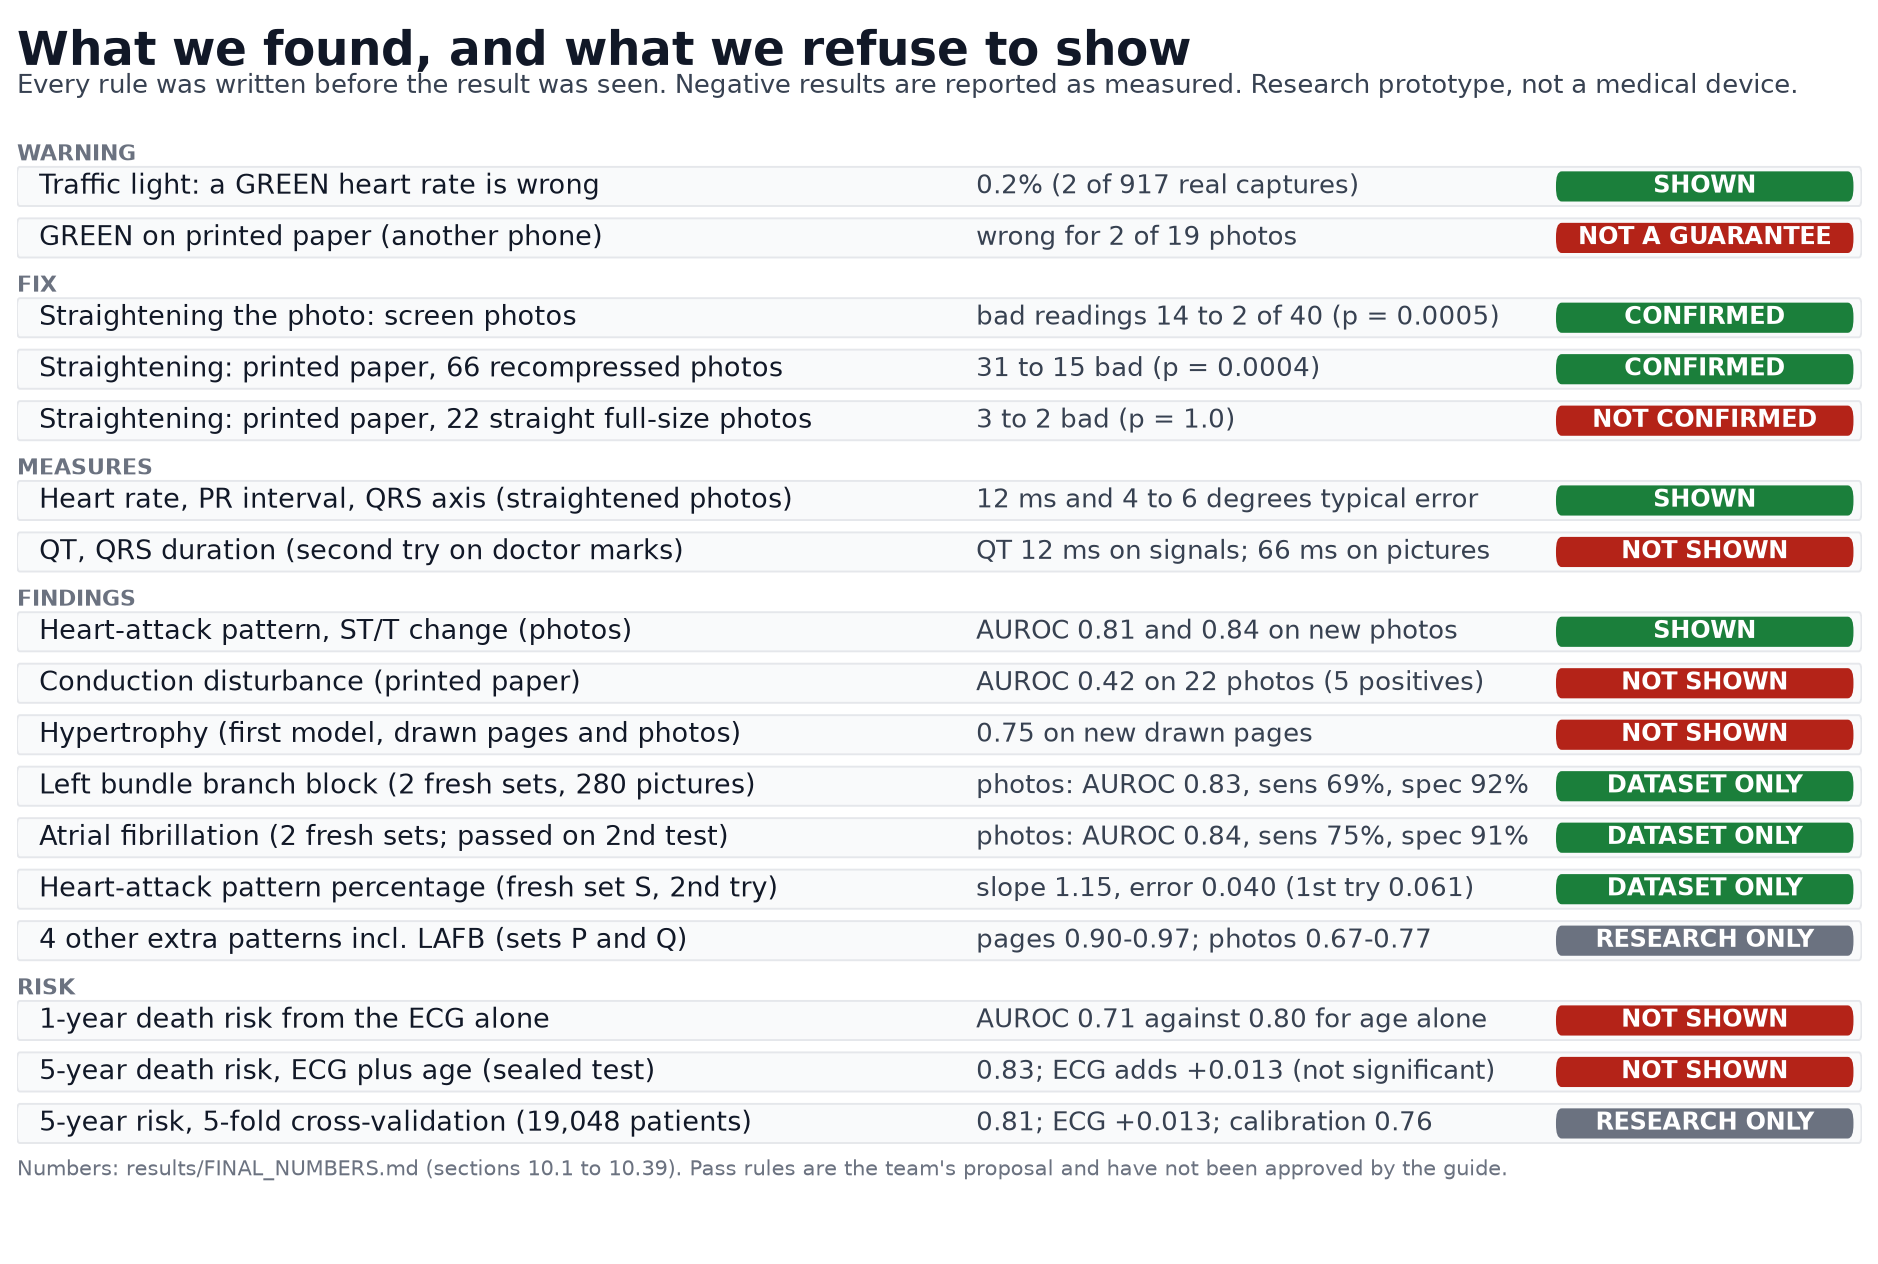
\includegraphics[width=0.78\textwidth]{figures/fig_results_at_a_glance.png}
\caption{Results at a glance: what was found, and what is not shown.}
\label{fig:glance}
\end{figure*}

Fig.~\ref{fig:glance} lists every result together with its verdict. 
Three findings stand out. First, the digitizer is more robust than expected: only very low resolution and heavy blur broke heart rate. Second, the picture cannot tell which pages will fail, but the digitized signal can; and the simplest effective fix on real photographs was geometric, flattening the page. Third, validating measurements one by one showed that heart rate, PR and axis can be read from straightened photographs, while QT, QRS duration and P- and T-wave amplitude cannot yet be read safely. The slope and tail checks matter: QRS duration had a typical error of 5--6~ms yet a bias of $+15$~ms on photos, and QT looked close on pages while compressing short values toward the mean, which would make a short QT look normal. These checks were fixed before the tests; relaxing them after a miss would have produced a passing but misleading result.

Printed paper from another phone was harder: GREEN readings were wrong for 2 of 19 straight photos and straightening was confirmed only on the recompressed set, so neither the light nor the page flattening transfers without limits. Networks trained only on public data read QRS duration on drawn pages but lost it on photos, and the mortality-risk pilots did not beat age alone (five years: 0.833 against 0.819, difference not significant) and did not survive digitization on simulated photos; a risk percentage from a phone photo of an ECG is not supported by our data. The traffic light adds a safety layer but also flags irregular rhythms, so RED does not mean a bad heart. Our results do not show that the tool helps patients, and the clinician study of selective prediction warns that abstaining can raise missed problems \cite{ref26}.

\section{Limitations}
Damage is simulated on computer-drawn pages and the digitizer was trained on a similar generator; only one digitizer was studied. Our own photos come from one phone and one laptop screen; printed paper was photographed by one other person with an unknown phone (messaging-app copies, uneven page coverage, patterned background), and the photos of a page are not independent. The pattern findings and the risk pilot were tested on drawn pages and photos of PTB-XL recordings, never on outcomes for photographs; the risk transfer check is not an outcome validation; the risk data are all-cause mortality from one Brazilian primary-care source and the score is driven largely by age. Real captures hold fewer than 100 wrong readings, so those results are descriptive, and several intervals treat images as independent. References are commercial algorithms, not expert annotations; the pass thresholds are our proposal and not approved by the guide. The traffic light was trained on simulated damage and flags irregular rhythms more often. Right-axis detection is not shown to work, and the PR safeguard for atrial fibrillation is a precaution calibrated on 14 cases. The sealed pages and photos used for the QRS and QT attempts were reused for P- and T-wave amplitude (no P or T result had been seen, and the methods were developed elsewhere). Early results labelled exploratory must not be read as confirmed; only the straightening fix was confirmed in tests whose rule was fixed in advance (on screen photos and on recompressed printed-paper photos, but not on the straight full-resolution printed-paper photos). The tool is a research prototype and not a medical device.

\section{Conclusion}
With a fixed open digitizer, only very low resolution and heavy blur made the heart rate wrong at a high rate; a score from the picture could not predict failure, but a traffic light from the digitized signal flagged most bad readings; flattening the photographed page cut bad readings from 14 to 2 of 40 in a confirmed test; and per-measurement validation accepted heart rate, PR and axis for straightened photos while rejecting QT, QRS duration and P- and T-wave amplitude. On printed paper from another phone straightening was confirmed only on the recompressed copies, networks trained on public data found two ECG patterns on new photos (conduction failed on printed paper) but could not read QRS duration or QT from them, and two mortality-risk pilots failed their rules and no risk is shown. Future work: other phones, paper and digitizers; expert annotations; methods that pass the slope check for QT, QRS and the P and T waves; a clinician study of whether the warning changes decisions.

\bibliographystyle{IEEEtran}
\bibliography{references}

\end{document}
